\newcommand{\minipagespace}[1]{
	\begin{minipage}[c]{#1\textwidth}
		\ 
	\end{minipage}
}

\section{Culling}

Der erste Weg eine Voxel Engine zu optimieren wird
offensichtlich, wenn man sich einen Würfel aus $8$
Voxels betrachtet. Dabei beobachten wir, dass
die Hälfte der Seiten der Voxels nach innen schauen
und somit nicht sichtbar sind. Wenn man die
Seitenlänge dieses Würfels verdoppelt, multipliziert
man die Oberfläche mit $4$ und das Volumen mit $8$.
Somit entstehen immer mehr Seiten, die nach innen
schauen, umso größer das Objekt ist. Also wird
dies bei großen Objekten dazu führen, dass die
meisten Seiten nicht sichtbar sind.

\begin{center}
\begin{figure}[ht]
	\minipagespace{0.04}
	\begin{minipage}[c]{0.4\textwidth}
		\begin{center}
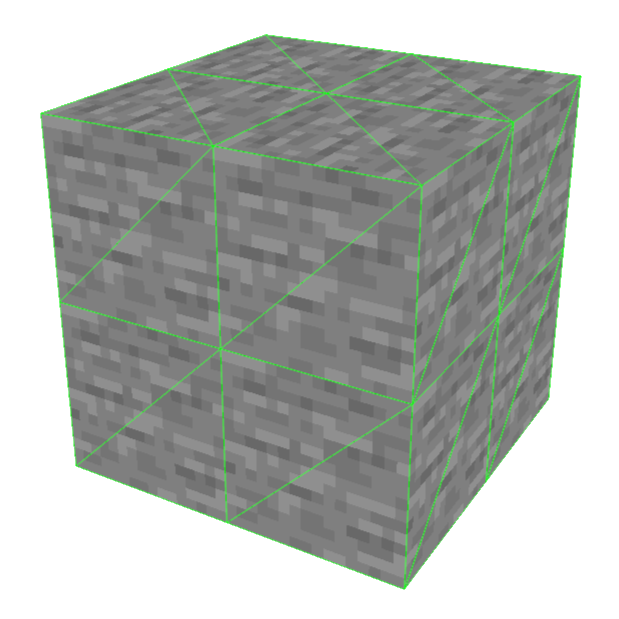
\includegraphics[width=1\textwidth]{assets/Culling/Opaque8Blocks.png}
		\end{center}
	\end{minipage}
	\minipagespace{0.09}
	\begin{minipage}[c]{0.4\textwidth}
		\begin{center}
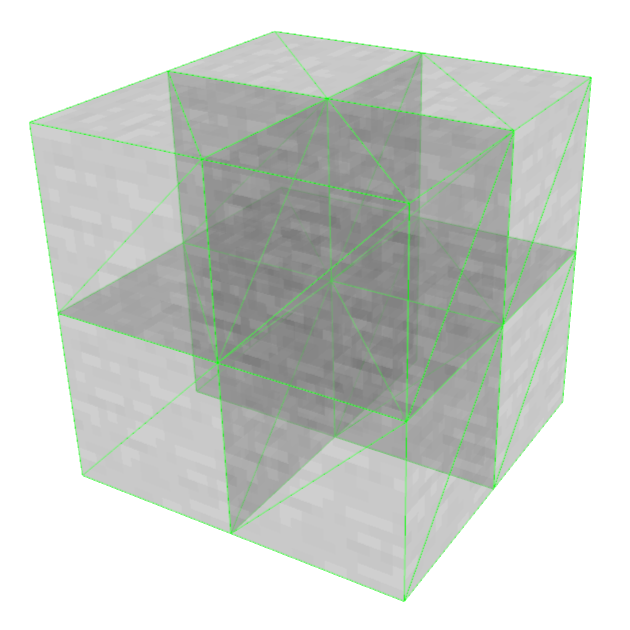
\includegraphics[width=1\textwidth]{assets/Culling/Transparent8Blocks.png}
		\end{center}
	\end{minipage}\hfill
\end{figure}
\end{center}

Mit \gqq{Culling} beschreibt man die Optimierung,
diese Seiten zu entfernen.

% TODO first basic culling impl
% TODO optimizing that with binary culling
